%======================================================================
\section{Full evaluation tables}
\label{app:tables}
%======================================================================

Tables~\ref{tab:evals_ks2d}--\ref{tab:evals_kolm0025} list every 2D model
evaluated in this work, including those that appear only in
Secs.~\ref{sec:results2d} and \ref{sec:failure}. Each entry gives the mean
$\DKY$ over initial conditions $\pm$ half the range, the number of
initial conditions, and the mean of the per-IC relative errors against
Table~\ref{tab:truth} (at Kolmogorov $\alpha=0.05$, $1\times$, each initial
condition against its matched-IC truth). Every individual evaluation,
with $\lambda_1$ and the number of positive exponents, is in
\texttt{artifacts/\allowbreak experiments/\allowbreak appendix\_D\_evaluations.csv}, generated with
these tables by \texttt{scripts/paper\_figures/tabD\_evaluations.py}. The
evaluation files themselves also store a truth value and an error; these
were computed against the truths available on the day of each
evaluation, several of which were later revised (Sec.~\ref{sec:truth_uncertainty}),
and are not used anywhere in this paper. The 1D evaluations are complete
in Table~\ref{tab:transfer1d}.

\para{The 12-channel models of Part~II.} The data assimilation experiments use a 12-channel sibling
of the 2D KS model, trained on noisy fields (Appendix~\ref{app:architecture}). Its $\DKY$ is $84.7$ at
$44^2$ and $188.5$ at $66^2$, against truths of $81.8$ and $192.5$ ($3.6\%$ and $2.1\%$); a 12-channel model
trained on clean fields gives $83.5$ and $190.4$ ($2.1\%$ and $1.1\%$), and the 6-channel model of Part~I
$1.7\%$ and $2.4\%$. Doubling the channels and training on noisy data leave the transfer of the dimension
within the spread of the truth runs (\texttt{artifacts/experiments/crop/p7c12*\_ks2d\_x*.json}; one
initial condition each).

Table~\ref{tab:spectra} gives, for the main-text models, the
reconstruction error of the autoencoder, the ratio of the decoded
rollout's standard deviation to the truth's, and the share of energy in
the lowest and highest wavenumber bands (1D and 2D KS: $|\bm k|<0.35$ and
$|\bm k|\ge1.4$; Kolmogorov flow: kinetic energy at $|\bm k|<1$ and
$|\bm k|\ge16$), from one initial condition and 1000 snapshots per size.

\begin{figure*}[htbp]
\centering
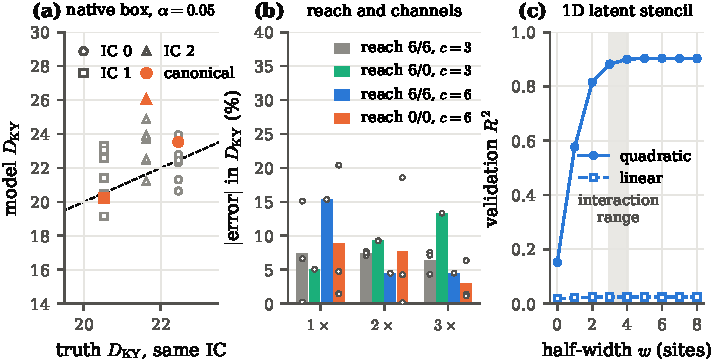
\includegraphics{figures/figC2_appendix_panels.pdf}
\caption{Supporting evidence. (a) Kolmogorov flow at $\alpha=0.05$, native
box: each model's $\DKY$ from one initial condition against the truth run
from the same initial condition (marker shape), for every model with
three native-size evaluations; filled: the canonical model; dashed: equality.
The truth varies by $\pm4.5\%$ across these initial conditions, single
models by $\pm1$--$12\%$. The models largely agree on the ordering, seven
of eight giving their largest value from IC~2, which the truth does not
share (its largest is from IC~0), so matching initial conditions removes
the truth's sampling noise but not the models'. (b) Reach and channel ablation at
$\alpha=0.05$, all trained on the same windows: encoder/decoder reach in
sites and number of channels; bars are means of $|$error$|$ over initial
conditions, dots individual initial conditions. (c) Interaction range of
the 1D latent dynamics: validation $R^2$ of one stencil, shared by all
sites, that predicts each site's one-step increment from the sites within
half-width $w$; the quadratic stencil saturates at $w=3$--$4$ sites
($19$--$25$ length units, shaded), the linear one explains almost
nothing (Sec.~\ref{sec:receptive}).}
\label{fig:appendix_panels}
\end{figure*}

\newcommand{\evalhead}[1]{model & description & #1 \\ \hline}
\newcommand{\evalnotes}{\par\footnotesize $^a$Trained on an $8\times8$-site
periodic box with the same architecture as the window-trained full-reach
models; the $\alpha=0.1$, $3\times$ value uses an unstandardized initial
condition, the only evaluation available. $^b$Narrow architecture
(encoder radius 1 over 2 layers, propagator window 1) trained on windows
of a $3\times$ periodic domain and evaluated on that domain.
$^\star$Main-text model.}

\begin{table*}[htbp]
\caption{2D KS: all evaluations. Columns: $44^2$, $66^2$, $88^2$ (no truth at $88^2$).}
\label{tab:evals_ks2d}
\widetabular{llccc}{\evalhead{$44^2$ & $66^2$ & $88^2$}
\tabinput{tables/tabD_ks2d}}
\evalnotes
\end{table*}

\begin{table*}[htbp]
\caption{Kolmogorov flow, $\alpha=0.1$: all evaluations (channel widths $1\times$, $2\times$, $3\times$).}
\label{tab:evals_kolm01}
\widetabular{llccc}{\evalhead{$1\times$ & $2\times$ & $3\times$}
\tabinput{tables/tabD_kolm01}}
\evalnotes
\end{table*}

\begin{table*}[htbp]
\caption{Kolmogorov flow, $\alpha=0.05$: all evaluations.}
\label{tab:evals_kolm005}
\widetabular{llccc}{\evalhead{$1\times$ & $2\times$ & $3\times$}
\tabinput{tables/tabD_kolm005}}
\evalnotes
\end{table*}

\begin{table*}[htbp]
\caption{Kolmogorov flow, $\alpha=0.025$: all evaluations.}
\label{tab:evals_kolm0025}
\widetabular{llccc}{\evalhead{$1\times$ & $2\times$ & $3\times$}
\tabinput{tables/tabD_kolm0025}}
\end{table*}

\begin{table}[htbp]
\caption{Reconstruction and decoded-rollout statistics of the main-text
models. ``recon.'': autoencoder error as a percentage of the field
variance; ``std'': decoded rollout standard deviation over the truth's;
the last two columns give the energy share (\%) in the lowest band for
truth / model rollout and in the highest band for truth /
reconstruction.}
\label{tab:spectra}
\begin{ruledtabular}\footnotesize
\begin{tabular}{llcccc}
system & size & recon. & std & low band & high band \\
\hline
\tabinput{tables/tabD_spectra}
\end{tabular}
\end{ruledtabular}
\end{table}
